
%----------------------------------------------------------------------------------------
%	PACKAGES AND OTHER DOCUMENT CONFIGURATIONS
%----------------------------------------------------------------------------------------

\documentclass[final]{beamer}

\usepackage[scale=1.24]{beamerposter} % Use the beamerposter package for laying out the poster

\usepackage{algorithm,algorithmic}
\usepackage{url}

\usetheme{confposter} % Use the confposter theme supplied with this template

\setbeamercolor{block title}{fg=blue,bg=white} % Colors of the block titles
\setbeamercolor{block body}{fg=black,bg=white} % Colors of the body of blocks
\setbeamercolor{block alerted title}{fg=white,bg=dblue!70} % Colors of the highlighted block titles
\setbeamercolor{block alerted body}{fg=black,bg=dblue!10} % Colors of the body of highlighted blocks
% Many more colors are available for use in beamerthemeconfposter.sty

%-----------------------------------------------------------
% Define the column widths and overall poster size
% To set effective sepwid, onecolwid and twocolwid values, first choose how many columns you want and how much separation you want between columns
% In this template, the separation width chosen is 0.024 of the paper width and a 4-column layout
% onecolwid should therefore be (1-(# of columns+1)*sepwid)/# of columns e.g. (1-(4+1)*0.024)/4 = 0.22
% Set twocolwid to be (2*onecolwid)+sepwid = 0.464
% Set threecolwid to be (3*onecolwid)+2*sepwid = 0.708

\newlength{\sepwid}
\newlength{\halfcolwid}
\newlength{\onecolwid}
\newlength{\twocolwid}
\newlength{\threecolwid}
\setlength{\paperwidth}{48in} % A0 width: 46.8in
\setlength{\paperheight}{36in} % A0 height: 33.1in
\setlength{\sepwid}{0.02\paperwidth} % Separation width (white space) between columns
\setlength{\halfcolwid}{0.13\paperwidth} % Width of one column
\setlength{\onecolwid}{0.3\paperwidth} % Width of one column
\setlength{\twocolwid}{0.464\paperwidth} % Width of two columns
\setlength{\threecolwid}{0.708\paperwidth} % Width of three columns
\setlength{\topmargin}{-0.6in} % Reduce the top margin size
%-----------------------------------------------------------

\usepackage{graphicx}  % Required for including images

\usepackage{booktabs} % Top and bottom rules for tables

%----------------------------------------------------------------------------------------
%	TITLE SECTION 
%----------------------------------------------------------------------------------------

\title{Web page comparison on post-load DOM trees} % Poster title

\author{Jonathan Thomas (Honors Capstone), Ayush Goel and Prof. Harsha Madhyastha} % Author(s)

\institute{University of Michigan} % Institution(s)

%----------------------------------------------------------------------------------------

\begin{document}

\addtobeamertemplate{block end}{}{\vspace*{0.5ex}} % White space under blocks
\addtobeamertemplate{block alerted end}{}{\vspace*{0.5ex}} % White space under highlighted (alert) blocks

\setlength{\belowcaptionskip}{0.5ex} % White space under figures
\setlength\belowdisplayshortskip{0.5ex} % White space under equations

\begin{frame}[t] % The whole poster is enclosed in one beamer frame

\begin{columns}[t] % The whole poster consists of three major columns, the second of which is split into two columns twice - the [t] option aligns each column's content to the top

\begin{column}{\sepwid}\end{column} % Empty spacer column

\begin{column}{\onecolwid} % The first column

%----------------------------------------------------------------------------------------
%	OBJECTIVES
%----------------------------------------------------------------------------------------

\begin{alertblock}{Problem}
Live code is always in a continuous state of improvement and being rewritten. As such, source code for web pages also changes drastically over time, and it is important to know what it really means for a web page to be the same as another or the same as a previous version of itself. 

\begin{columns}
\begin{column}{\halfcolwid}
The main entity we are concerned with is the Document Object Model (DOM) tree, which keeps track of the structure of the web page at a high level. 
\end{column}

\begin{column}{\halfcolwid} % Begin a column which is two columns wide (column 2)
\begin{figure}
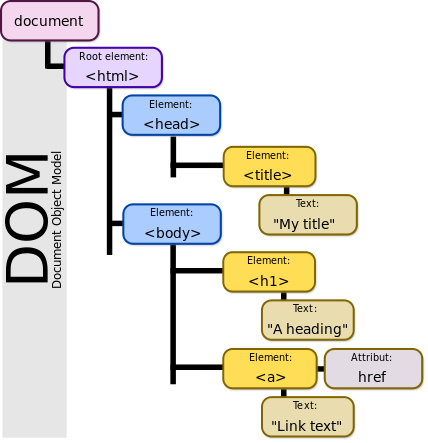
\includegraphics[width=0.6\linewidth]{dom.png}
\caption{An example DOM}
\end{figure}
\end{column}
\end{columns}
There is a need for an approach and implementation of a more useful way to check differences between two web pages than a naive diff of the source text or checking for DOM tree equality. We also wish to get a better understanding for how the DOM differs over different sites as well as environments, which will be explained below.
\end{alertblock}

%----------------------------------------------------------------------------------------
%	OBJECTIVE
%----------------------------------------------------------------------------------------

\begin{block}{Objective}
In this project, I wrote a correctness checker to determine how similar two web pages are from the perspective of a user visiting either page by creating a program to compare the resulting post-load DOM trees of loading two web pages and can quantify how similar they are. Using this tool, we aim to form a better idea of how real web pages change. 

The major steps for this project included:
\begin{itemize}
    \item Loading a site, dumping the post-load DOM and parsing this into a virtual DOM tree that can be manipulated effectively. 
    \item Comparing the two trees and reporting the differences.
    \item Automating and batching this process with several websites and across different environments and graphing the results.
\end{itemize}
\end{block}

%----------------------------------------------------------------------------------------
%	METHODS
%----------------------------------------------------------------------------------------
\vspace{-0.5cm}
\begin{block}{Methodology}
To evaluate the appearance of the DOM in addition to the structure, we make a first pass over the source code and serialize the computed CSS styles into the DOM to use as an additional check. 

In addition to comparing two loads of the same web page in a standard live setup, we wanted to explore how the DOM changes in a replay environment using the mahimahi tool \cite{netravali_sivaraman_winstein_das_goyal_balakrishnan_2014}. After recording replay data for $\sim 100$ randomly chosen websites, we performed the comparison within these replay environments. We also constructed modified versions of the replay environments by manually removing sources of non-determinism from the included JavaScript scripts. 
\end{block}

%----------------------------------------------------------------------------------------

\end{column} % End of the first column

\begin{column}{\sepwid}\end{column} % Empty spacer column

\begin{column}{\onecolwid} % Begin a column which is two columns wide (column 2)

%----------------------------------------------------------------------------------------
%	ALGORITHM
%----------------------------------------------------------------------------------------

%\begin{block}{Comparison Algorithm}

%For the comparison algorithm, we check the longest common subsequence formed by two nodes' children, and only comparing the matching nodes. While this algorithm has greater time complexity ($O(n^2)$ compared to $O(n)$ for a naive recursive method), the DOM trees are usually no greater than 1000 nodes, and the comparison still ran fairly quickly. Finally, to check our results and strengthen the existing comparison, we added comparisons of the network requests fired by each load as well as the resulting screenshots of the websites after loading.

%\vspace{0.75cm}
%\begin{algorithm}[H]
%\begin{algorithmic}
%% \IF{!compare\_attrs(left\_root, right\_root)}
%\FOR{$i=1$ to $N$}
%\FOR{$j=1$ to $JJJJ$}
%\STATE $energy[i*JJJ+j] =$ 
%$ interpolate(AAA[i*JJJ+j], ZZZ)$
%\ENDFOR
%\ENDFOR
%\end{algorithmic}
%\caption{pseudocode for DOM comparison}
%\label{alg:seq}
%\end{algorithm}


% For the DOM comparison, we check the number of nodes compared and report the number of unmatched nodes in the maximum size tree. For comparing the fired network requests, we again report the number of unmatched network requests as a fraction of the total (discarding duplicates and requests that do not affect the DOM). Finally, to compare the screenshots, we used a simple image edit distance library and normalized this with respect to the image size. 

%\end{block}

%----------------------------------------------------------------------------------------
%	RESULTS
%----------------------------------------------------------------------------------------

\begin{block}{Results}

First, we justify why a smarter DOM comparison is necessary. The following graph compares the differences detected in a naive algorithm vs. our algorithm in comparing a suite of live web pages.

\begin{figure}
\vspace{0.5cm}
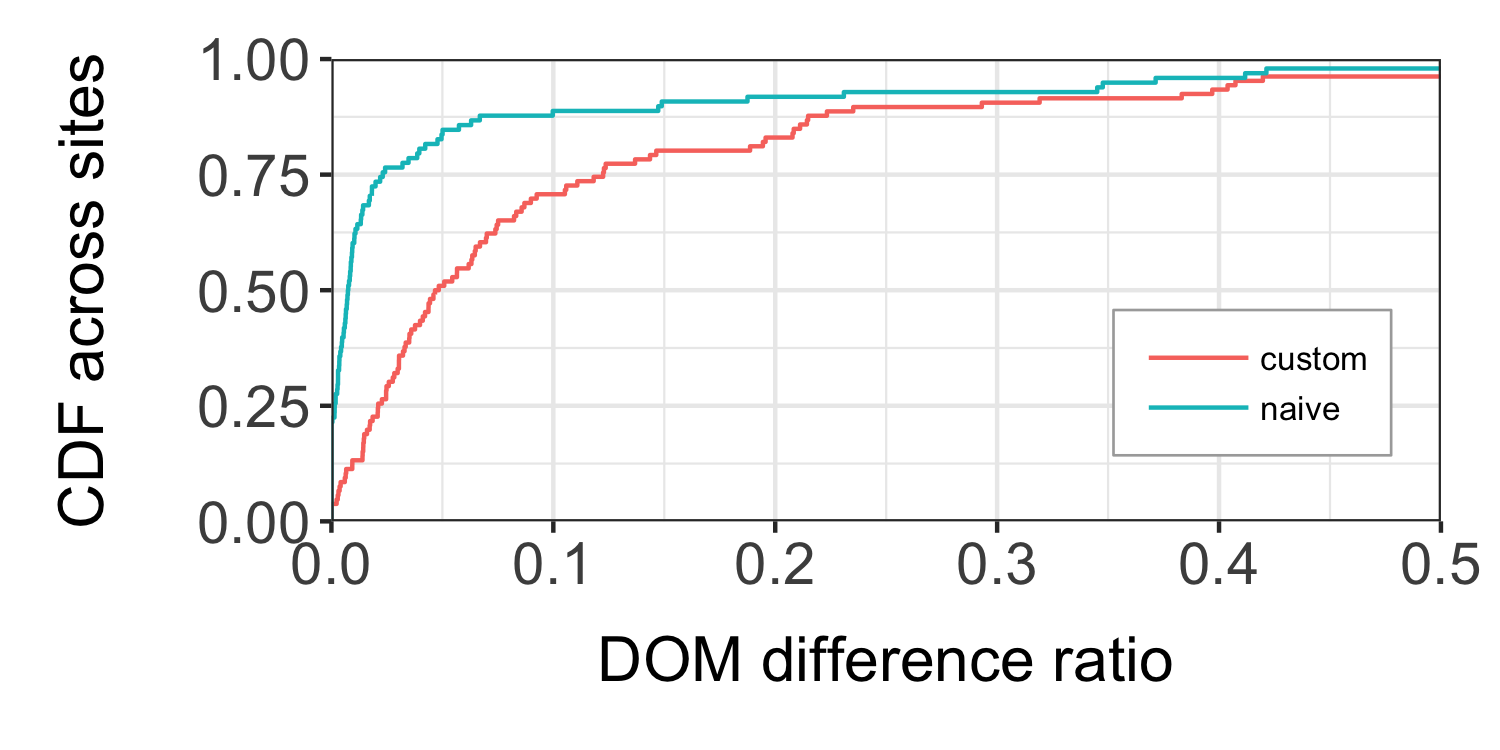
\includegraphics[width=0.6\linewidth]{naive_comparison_plot.png}
\caption{How our comparison performs compared to a naive approach}
\end{figure}

As seen, our approach identifies many additional differences and gives a higher signal for if a web page has changed. 

Having established the viability of this approach, we now compare the differences between the three classes of comparisons: comparison with live loads, loads within a replay environment, and reloads within the modified replay environment.

\begin{figure}
\vspace{0.5cm}
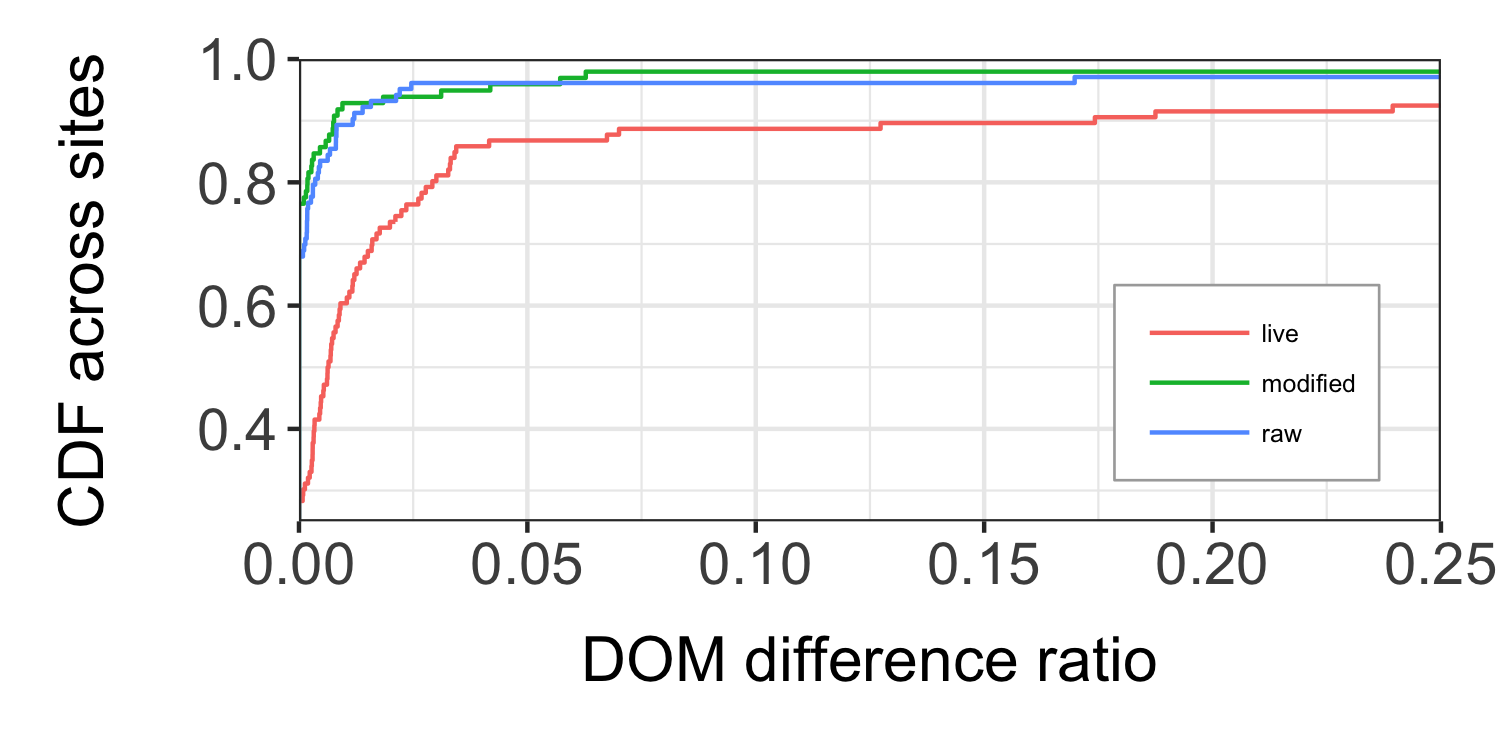
\includegraphics[width=0.9\linewidth]{dom_plot.png}
\caption{DOM comparison across environments}
\end{figure}

Finally, we show how the logged network requests change across the different environments for reference.

\begin{figure}
\vspace{0.5cm}
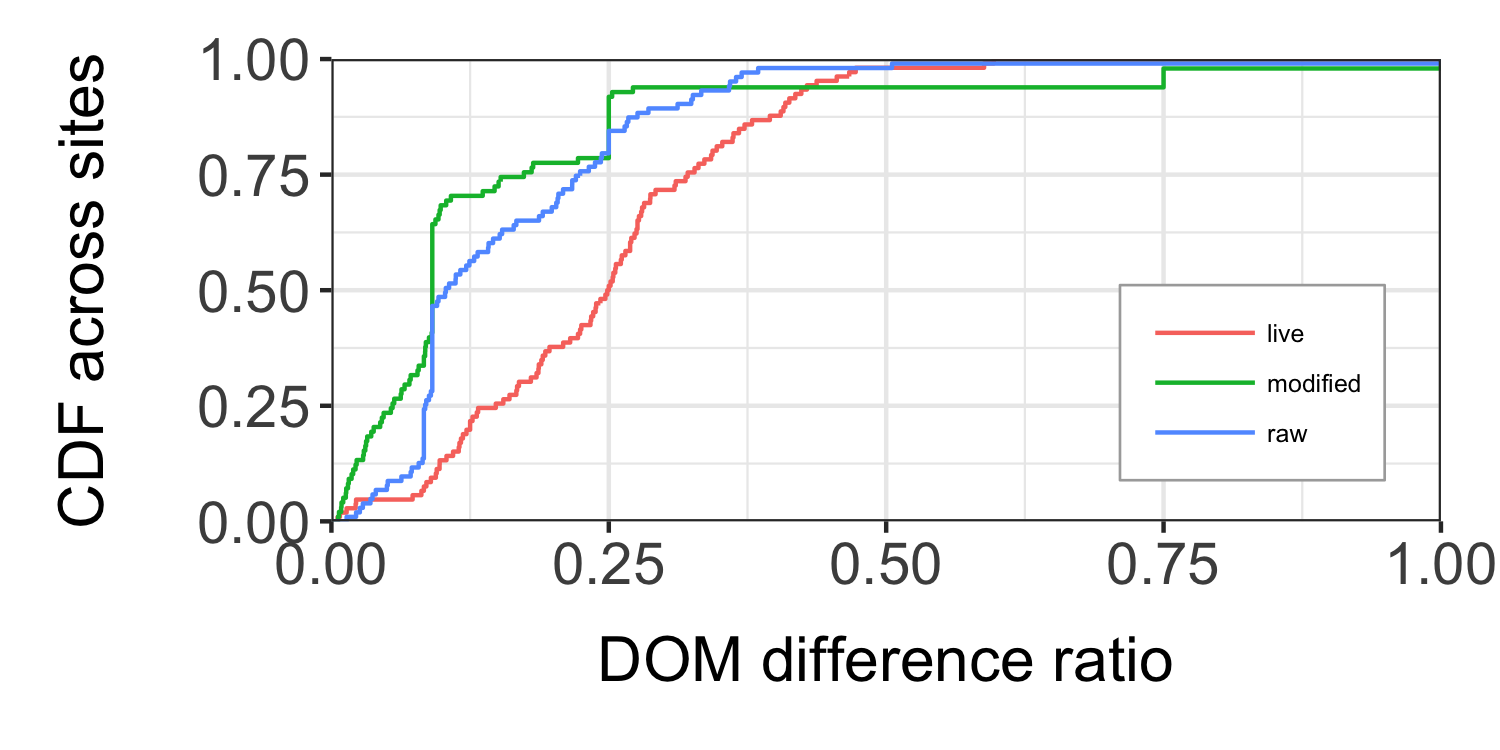
\includegraphics[width=0.8\linewidth]{network_plot.png}
\caption{Network request comparison across environments}
\end{figure}

\end{block}

%----------------------------------------------------------------------------------------

\end{column} % End of the second column

\begin{column}{\sepwid}\end{column} % Empty spacer column

\begin{column}{\onecolwid} % The third column

%----------------------------------------------------------------------------------------
%	DISCUSSION
%----------------------------------------------------------------------------------------

\begin{block}{Discussion}

The results show that more than 70\% of the  live web pages sampled change across back-to-back loads. Existing work supports the general trend of this data of only roughly 22\% of websites having the same DOM structure on back to back loads \cite{ruamviboonsuk_netravali_uluyol_madhyastha_2017}. 

Additionally, while the replay environment helps decrease the detected changes in the DOM as well as in the network requests sent, there are still sources of non-determinism that cause the DOM to change. In the modified replay environments supplied, we see less change, but there are still sources of differences present that are being investigated. 

\end{block}

%----------------------------------------------------------------------------------------
%	CONCLUSION
%----------------------------------------------------------------------------------------

\begin{block}{Next Steps}

Future questions for extending this project include optimization of the existing tool, a better characterization of the types of differences that appear, and extending the modified replay environment to account for more sources of non-determinism. 
%A development of a unified metric that incorporates both the DOM changes and network request changes and accurately reports the differences would be useful. 

Another application of this would be for further use in the field of web page optimization research. This project could be used to evaluate the correctness of existing work, where rewriting source code is common to gain improvements in speed and memory usage. This project provides useful information to users to determine how their rewrites have affected the content of the rewritten web pages.
\end{block}

%----------------------------------------------------------------------------------------
%	REFERENCES
%----------------------------------------------------------------------------------------

\begin{block}{References}
\vspace{-0.5cm}
\nocite{*} % Insert publications even if they are not cited in the poster
\small{\bibliographystyle{unsrt}
\bibliography{sample}}

\end{block}

%----------------------------------------------------------------------------------------
%	ACKNOWLEDGEMENTS
%----------------------------------------------------------------------------------------

%\setbeamercolor{block title}{fg=red,bg=white} % Change the block title color

%----------------------------------------------------------------------------------------
%	CONTACT INFORMATION
%----------------------------------------------------------------------------------------

\begin{alertblock}{Acknowledgements}

\small{\rmfamily{I would like to thank Prof. Harsha Madhyastha, Ayush Goel, and the Engineering Honors Program for guiding and helping me to complete this project.
}} \\

\begin{itemize}
\item Email: \href{mailto:jonthoma@umich.edu}{jonthoma@umich.edu}
\end{itemize}
\end{alertblock}

\vspace{-2cm}
\begin{center}
\begin{figure}

\includegraphics[width=0.4\linewidth]{CoE-Honors-vert.png}
\end{figure}
\end{center}

%\begin{columns}
%\begin{column}{\halfcolwid}
%\begin{figure}
%\includegraphics[width=\linewidth]{logo.png}
%\caption{Replace with EECS logo}
%\end{figure}
%\end{column}

%\begin{column}{\halfcolwid} % Begin a column which is two columns wide (column 2)
%\begin{figure}
%
\includegraphics[width=\linewidth]{CoE-Honors-vert.png}
%\end{figure}
%\end{column}
%\end{columns}

%----------------------------------------------------------------------------------------

\end{column} % End of the third column

\end{columns} % End of all the columns in the poster

\end{frame} % End of the enclosing frame

\end{document}
